\documentclass[11pt]{article}

\usepackage[portuguese]{babel}
\usepackage[utf8]{inputenc}
\usepackage{amsmath}
\usepackage{graphicx}
\usepackage{float}
\usepackage{subfig}
\usepackage{fixltx2e}
\usepackage[bottom]{footmisc}
\usepackage{listings}
\usepackage{color} 
\usepackage[usenames,dvipsnames]{xcolor}
\usepackage[colorinlistoftodos]{todonotes}
\usepackage[font=footnotesize]{caption}

\setcounter{tocdepth}{3}

\numberwithin{equation}{section}

\linespread{1.3}
\usepackage{indentfirst}
\usepackage[top=2cm, bottom=2cm, right=2.3cm, left=2.3cm]{geometry}
\addto\captionsportuguese{\renewcommand{\contentsname}{Índice}}

\begin{document}

\begin{titlepage}
\begin{center}

\hfill \break
\hfill \break


\includegraphics[width=0.3\textwidth]{./logo}~\\[1cm] 

\textsc{\LARGE Instituto Superior Técnico}\\[0.25cm]
\textsc{\Large Mestrado Integrado em Engenharia Electrotécnica e de Computadores}\\[1.8cm]
\textsc{\huge Electrónica Rápida}\\[0.25cm]

\vspace{6mm}

{\huge \bfseries Projecto e Simulação de Amplificadores Lineares para Altas Frequências\\[1cm]}

\begin{tabular}{ l l }
Guilherme Branco Teixeira & \hspace{2mm} n.º 70214 \\
Maria Margarida Dias dos Reis & \hspace{2mm} n.º 73099 \\
Nuno Miguel Rodrigues Machado & \hspace{2mm} n.º 74236
\end{tabular}

\vspace{7mm}

Grupo n.º 2 de quarta-feira das 11h00 - 12h30

\vfill

{\large Lisboa, 25 de Abril de 2015} 

\end{center}
\end{titlepage}

\pagenumbering{gobble}
\clearpage

\tableofcontents
\pagebreak

\clearpage
\pagenumbering{arabic}

\section{Introdução}

O objectivo deste laboratório é estudar técnicas de projecto de amplificadores lineares de alta frequência, análise das suas caracteristicas (estabilidade, ganho, adaptação e factor de ruído) e comportamentos. A caracterização dos dispositivos do amplificador será realizada através dos pârametros distribuidos (Parâmetros S).

Iremos utilizar um transistor da Hewlett-Packard(hp) ATF-35176. É um transistor que utiliza tecnologia PHEMT (Pseudomorphic High Mobility Transistor), preparado para trabalhar em altas frequências.

\section{Plano de Trabalhos}

Foi seguido o plano de trabalhos descrito no enunciado do laboratório.

As especificações do amplificador a construir podem ser consultadas na Tabela, tal como as caracteristicas do substrato plástico para alta-frequência da Taconic (TLY -3-0310-CH/CH), sobre qual o transistor irá ser implantado. 

\begin{tabular}{|c|c|c|c|c|c|c|c|}
	\hline  $ G_{T} $ & $ V_{DS} $ & $ I_{DS} $ & $ R_{G} $/$ R_{C} $ & er & h & t & sigma  \\ 
	\hline  $ G_{Tmax} $ & 1.5 V & 20 mA & 50 & 2.3 & 0.78 & 0.018 & 0.001  \\ 
	\hline 
\end{tabular} 


Numa primeira fase do laboratório irá ser projectado e simulado o amplificador uniandar com linhas simétricas. Na segunda fase, o amplificador irá ser projectado com tecnologia de microfita.

\subsection{Projecto de um amplificador uniandar}

\subsubsection{a) Projecto do amplificador com linhas ideais}

Nesta primeira fase o amplificador irá ser constituido pelo transistor descrito anteriormente, no entanto, todos os dispositivos utilizados no seu projecto e simulação serão dispositivos ideais, esta fase inicial tem como objectivo definir os parâmetros do amplificador que permitem obter as especificações pedidas.

\paragraph{PFR.}

Em primeiro lugar será feita uma análise DC ao transistor que tenha em vista obter o ponto de funcionamento em repouso especificado, o circuito que nos permitiu alcançar essa análise é o que se vê na Figura \ref{fig:Circuito_0}.

\begin{figure}[H]
	\centering
	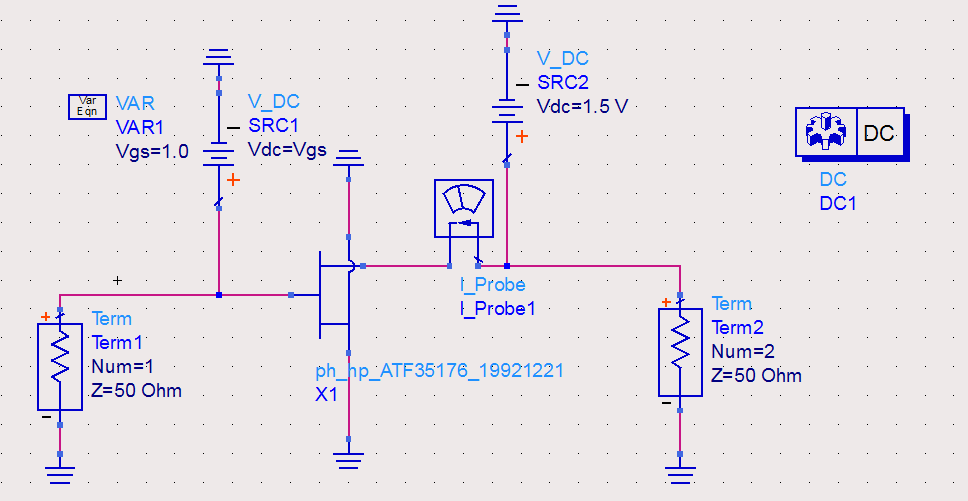
\includegraphics[width=0.7\textwidth]{./imagens/Circuito_0}~\\
	\caption{Circuito utilizado para obter o PFR desejado}
	\label{fig:Circuito_0}
\end{figure}

A análise DC servirá para descobrir o valor de $ V_{GS} $ correspondente ao PFR desejado. No circuito da Figura \ref{fig:Circuito_0} existe um componente denominado de \textit{I\_Probe} que tem como objectivo controlar o valor de $ I_{D} $ à medida que o valor de $ V_{GS} $ varia. Um excerto dos resultados desta análise podem ser consultados na Figura \ref{fig:VGS}, onde se pode concluir que o valor da tensão  $ V_{GS} $ que melhor corresponde a uma corrente  $ I_{D} $ de $ 20 mA $ ($20.03 mA$) é de  $ -0.277 V $ .

\begin{figure}[H]
	\centering
	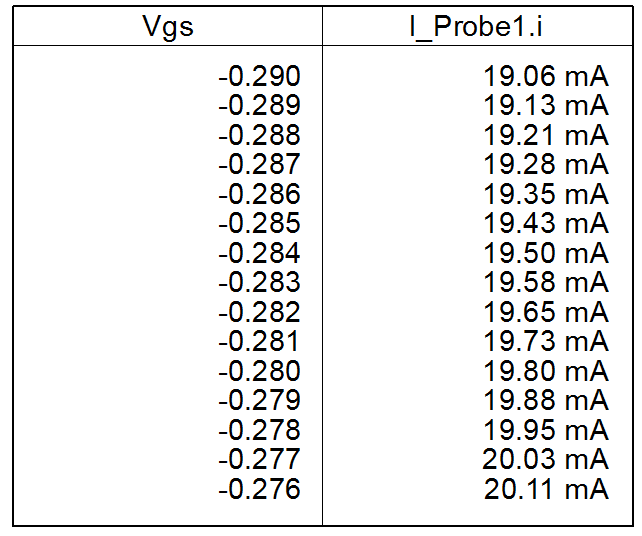
\includegraphics[width=0.35\textwidth]{./imagens/Vgs}~\\
	\caption{Circuito utilizado para obter o PFR desejado}
	\label{fig:VGS}
\end{figure}

Podemos agora continuar a projectar o amplificador, visto que temos agora todos os dados relevantes do ponto de funcionamento em repouso.

\paragraph{Análise de alta-frequência}

Com o transistor no PFR desejado, é preciso construir um novo circuito que contenha condensadores e bobines ideais, DC\_Block e DC\_Feed respectivamente, para que seja possível realizar a simulação dos Parametros S.


\paragraph{3.}
\paragraph{4.}

\subsubsection{b) Projecto do amplificador utilizando tecnologia microfita}

\subsection{Concretização do amplificador em tecnologia de microfita}

\subsubsection{a) Introdução de elementos que simulam descontinuidades nas linhas}

\subsubsection{b) Substituição do transístor e condensadores}

\section{Conclusões}

\end{document}